\documentclass[twoside]{article}
\setlength{\oddsidemargin}{0.25 in}
\setlength{\evensidemargin}{-0.25 in}
\setlength{\topmargin}{-0.6 in}
\setlength{\textwidth}{6.5 in}
\setlength{\textheight}{8.5 in}
\setlength{\headsep}{0.75 in}
\setlength{\parindent}{0 in}
\setlength{\parskip}{0.1 in}

\usepackage{graphicx}
\usepackage{url}

%
% The following commands sets up the lecnum (lecture number)
% counter and make various numbering schemes work relative
% to the lecture number.
%
\newcounter{lecnum}
\renewcommand{\thepage}{\thelecnum-\arabic{page}}
\renewcommand{\thesection}{\thelecnum.\arabic{section}}
\renewcommand{\theequation}{\thelecnum.\arabic{equation}}
\renewcommand{\thefigure}{\thelecnum.\arabic{figure}}
\renewcommand{\thetable}{\thelecnum.\arabic{table}}
\newcommand{\dnl}{\mbox{}\par}

%
% The following macro is used to generate the header.
%
\newcommand{\lecture}[4]{
  \pagestyle{myheadings}
  \thispagestyle{plain}
  \newpage
  \setcounter{lecnum}{#1}
  \setcounter{page}{1}
  \noindent
  \begin{center}
  \framebox{
     \vbox{\vspace{2mm}
   \hbox to 6.28in { {\bf COMPSCI~590S~~~Systems for Data Science
                       \hfill Fall 2016} }
      \vspace{4mm}
      \hbox to 6.28in { {\Large \hfill Lecture #1: #2  \hfill} }
      \vspace{2mm}
      \hbox to 6.28in { {\it Lecturer: #3 \hfill Scribe(s): #4} }
     \vspace{2mm}}
  }
  \end{center}
  \markboth{Lecture {#1}: #2}{Lecture {#1}: #2}
  \vspace*{4mm}
}

%
% Convention for citations is authors' initials followed by the year.
% For example, to cite a paper by Leighton and Maggs you would type
% \cite{LM89}, and to cite a paper by Strassen you would type \cite{S69}.
% (To avoid bibliography problems, for now we redefine the \cite command.)
%
\renewcommand{\cite}[1]{[#1]}

% \input{epsf}

%Use this command for a figure; it puts a figure in wherever you want it.
%usage: \fig{NUMBER}{FIGURE-SIZE}{CAPTION}{FILENAME}
\newcommand{\fig}[4]{
           \vspace{0.2 in}
           \setlength{\epsfxsize}{#2}
           \centerline{\epsfbox{#4}}
           \begin{center}
           Figure \thelecnum.#1:~#3
           \end{center}
   }

% Use these for theorems, lemmas, proofs, etc.
\newtheorem{theorem}{Theorem}[lecnum]
\newtheorem{lemma}[theorem]{Lemma}
\newtheorem{proposition}[theorem]{Proposition}
\newtheorem{claim}[theorem]{Claim}
\newtheorem{corollary}[theorem]{Corollary}
\newtheorem{definition}[theorem]{Definition}
\newenvironment{proof}{{\bf Proof:}}{\hfill\rule{2mm}{2mm}}

% Some useful equation alignment commands, borrowed from TeX
\makeatletter
\def\eqalign#1{\,\vcenter{\openup\jot\m@th
 \ialign{\strut\hfil$\displaystyle{##}$&$\displaystyle{{}##}$\hfil
     \crcr#1\crcr}}\,}
\def\eqalignno#1{\displ@y \tabskip\@centering
 \halign to\displaywidth{\hfil$\displaystyle{##}$\tabskip\z@skip
   &$\displaystyle{{}##}$\hfil\tabskip\@centering
   &\llap{$##$}\tabskip\z@skip\crcr
   #1\crcr}}
\def\leqalignno#1{\displ@y \tabskip\@centering
 \halign to\displaywidth{\hfil$\displaystyle{##}$\tabskip\z@skip
   &$\displaystyle{{}##}$\hfil\tabskip\@centering
   &\kern-\displaywidth\rlap{$##$}\tabskip\displaywidth\crcr
   #1\crcr}}
\makeatother

% **** IF YOU WANT TO DEFINE ADDITIONAL MACROS FOR YOURSELF, PUT THEM HERE:



% Some general latex examples and examples making use of the
% macros follow.

\begin{document}

%FILL IN THE RIGHT INFO.
%\lecture{**LECTURE-NUMBER**}{**DATE**}{**LECTURER**}{**SCRIBE**}
\lecture{13}{Google File System, BigTable}{Emery Berger}{Arjun Sreedharan,Yuchen Cai}



\section{Google File System}

\subsection{Lease}
There need to be a mechanism to control client access to chunks. The naive approach here would be to use locks. But, locks are not tolerant to failures. Since there is a possibility that the client can die before releasing a lock it acquired, the Master will need to store all modifications made by the client and rollback them in the event of a failure. Instead GFS uses leases. Lease is a time limited granting of exclusive control of a chunk to a client. Once this lease expires, the Master is free to hand over the lease to another client. Therefore right before committing to a chunk, the client has to check again if it still holds the lease. Leases are also used in Bigtables.

\subsection{Record append}
Record append is an atomic append operation provided by GFS. The client specifies only the data and it is appended to the end of the file. All writes go to exactly one of the many replicas. It establishes an order of replicas for the chunks to be written to, and therefore maintains deterministic ordering. Record append assumes idempotent operations. Therefore, the same update can happen more than once. It follows a weakened append semantics - not everything is in order, not compulsorily one after another, but makes sure data is consistent and not scrambled.


\section{Bigtable}
Bigtable is a sparse, persistent, distributed NoSQL data storage developed by Google.\\
Apache equivalent of Bigtable: HBase.

\subsection{Data model}
Generally, NoSQL datadases store data as simple \textit{key} $\,\to\,$ \textit{value} pairs. Bigtable's data model is a generalization of such data storage systems. Here, the map is indexed by a row key, column key, and a timestamp: \textit{(row:string, column:string, time:int64)} $\,\to\,$ \textit{(value:string)}\\


\begin{tabular}{|c|c|c|c||c|}
\hline
Column1 & Column2 & ... & ColumnN & Value \\
\hline
        &         &     &         &       \\
\hline
        &         &     &         &       \\
\hline
        &         &     &         &       \\
\hline
\end{tabular}
Fig: A logical overview of Bigtable rows

A general key-value store may emulate this by jamming all columns to create a composite key. Bigtables do not do this because the user may only be interested in the data in only some of the columns, and therefore a more performant lookup is possible. Bigtables are sparse data stores, which means they are expected to have a lot of cells with no data. Using timestamps, different versions of a cell are maintained in most recent first order. The number of timestamped versions depend on a threshold set. The threshold specifies either that only the last \textit{n} versions of a cell be kept, or that only new enough versions be kept. The columns are grouped as families, and each column is identified as a pair \textit{(family: qualifier)}. The row IDs are sorted and split into different groups called \textit{tablets}. This lets BigTable take advantage of locality of data. This model however performs poorly on updates. It follows a \textit{write few read many model}.

\subsection{Tablet}
Each tablet contains one or more SSTables. SSTable (Sorted String Table) is a file format that provides an immutable, ordered key-value map. An SSTable contains multiple blocks (or chunks) and an index to locate the blocks. These chunks are of size 64KB each. The SSTable index stores ranges of rows and is loaded into the main memory for fast lookup. SSTables use binary search within the block for finding rows. Additionally, the recently committed updates are stored in memory in a sorted buffer called \textit{memtable}. When the memtable size reaches a threshold, it is frozen and converted to an SSTable. Bigtable uses a distributed lock service named Chubby for handling synchronization issues. Chubby runs on the Paxos algorithm and uses the lease mechanism.
\begin{figure}[h]
\centering
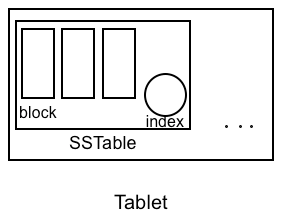
\includegraphics[width=0.5\linewidth]{tablet}
\caption[]{Tablet structure}
\end{figure}

\subsection{Block map}
When there are a lot of tablets, looking up tablets is a difficult task. To accomplish this, Big table uses a three-level block map. This works very similar to how a file system maps a file to its blocks.

\end{document}
